%%
%% Copyright 2007, 2008, 2009 Elsevier Ltd
%%
%% This file is part of the 'Elsarticle Bundle'.
%% ---------------------------------------------
%%
%% It may be distributed under the conditions of the LaTeX Project Public
%% License, either version 1.2 of this license or (at your option) any
%% later version.  The latest version of this license is in
%%    http://www.latex-project.org/lppl.txt
%% and version 1.2 or later is part of all distributions of LaTeX
%% version 1999/12/01 or later.
%%
%% The list of all files belonging to the 'Elsarticle Bundle' is
%% given in the file `manifest.txt'.
%%

%% Template article for Elsevier's document class `elsarticle'
%% with numbered style bibliographic references
%% SP 2008/03/01
%%
%%
%%
%% $Id: elsarticle-template-num.tex 4 2009-10-24 08:22:58Z rishi $
%%
%%
\documentclass[preprint,12pt,3p]{elsarticle}

%% Use the option review to obtain double line spacing
%% \documentclass[preprint,review,12pt]{elsarticle}

%% Use the options 1p,twocolumn; 3p; 3p,twocolumn; 5p; or 5p,twocolumn
%% for a journal layout:
%% \documentclass[final,1p,times]{elsarticle}
%% \documentclass[final,1p,times,twocolumn]{elsarticle}
%% \documentclass[final,3p,times]{elsarticle}
%% \documentclass[final,3p,times,twocolumn]{elsarticle}
%% \documentclass[final,5p,times]{elsarticle}
%% \documentclass[final,5p,times,twocolumn]{elsarticle}

%% if you use PostScript figures in your article
%% use the graphics package for simple commands
%% \usepackage{graphics}
%% or use the graphicx package for more complicated commands
%% \usepackage{graphicx}
%% or use the epsfig package if you prefer to use the old commands
%% \usepackage{epsfig}

%% The amssymb package provides various useful mathematical symbols
\usepackage{amssymb}
\usepackage[T2A]{fontenc}
\usepackage[utf8]{inputenc}
\usepackage[russian]{babel}
\usepackage{bm}

\usepackage{graphicx, epsfig}
\usepackage{graphicx}
\graphicspath{ {images/} }
\usepackage{bbding}

\usepackage{amsmath, multirow}
\usepackage{graphicx}
\usepackage{subfig}

%% The amsthm package provides extended theorem environments
\usepackage{amsthm}

%% The lineno packages adds line numbers. Start line numbering with
%% \begin{linenumbers}, end it with \end{linenumbers}. Or switch it on
%% for the whole article with \linenumbers after \end{frontmatter}.
%% \usepackage{lineno}

%% natbib.sty is loaded by default. However, natbib options can be
%% provided with \biboptions{...} command. Following options are
%% valid:

%%   round  -  round parentheses are used (default)
%%   square -  square brackets are used   [option]
%%   curly  -  curly braces are used      {option}
%%   angle  -  angle brackets are used    <option>
%%   semicolon  -  multiple citations separated by semi-colon
%%   colon  - same as semicolon, an earlier confusion
%%   comma  -  separated by comma
%%   numbers-  selects numerical citations
%%   super  -  numerical citations as superscripts
%%   sort   -  sorts multiple citations according to order in ref. list
%%   sort&compress   -  like sort, but also compresses numerical citations
%%   compress - compresses without sorting
%%
%% \biboptions{comma,round}

% \biboptions{}

\usepackage{etoolbox}
% \patchcmd{<cmd>}{<search>}{<replace>}{<success>}{<failure>}
\patchcmd{\abstract}{Abstract}{Аннотация}{}{}
\patchcmd{\keyword}{Keywords}{Ключевые слова}{}{}


%\journal{Nuclear Physics B}
\makeatletter
\def\ps@pprintTitle{%
 \let\@oddhead\@empty
 \let\@evenhead\@empty
 \def\@oddfoot{}%
 \let\@evenfoot\@oddfoot}
\makeatother

\begin{document}

\begin{frontmatter}

\title{Формулировка и решение задачи оптимизации, сочетающей классификацию и регрессию, для оценки энергии связывания белка и маленьких молекул}

% \title{Sample article to present \texttt{elsarticle} class\tnoteref{label0}}
% \tnotetext[label0]{This is only an example}

\author{Илья Игашов}
% \altaffiliation[Also at ]{Physics Department, XYZ University.}%Lines break automatically or can be forced with \\
\author{Сергей Грудинин}%
% \email{Second.Author@institution.edu.}
%\affiliation{ 
%Authors' institution and/or address%\\This line %break forced with \textbackslash\textbackslash
%}%

\author{Мария Кадукова}
% \homepage{http://www.Second.institution.edu/~Charlie.Author.}
%\affiliation{%
%Second institution and/or address%\\This line break forced% with \\
%}%
\author{В.В. Стрижов}

% \author[label1,label2]{Author One\corref{cor1}\fnref{label3}}
% \address[label1]{Address One}
% \address[label2]{Address Two\fnref{label4}}

% \cortext[cor1]{I am corresponding author}
% \fntext[label3]{I also want to inform about\ldots}
% \fntext[label4]{Small city}

% \ead{author.one@mail.com}
% \ead[url]{author-one-homepage.com}

% \author[label5]{Author Two}
% \address[label5]{Some University}
% \ead{author.two@mail.com}

% \author[label1,label5]{Author Three}
% \ead{author.three@mail.com}

\begin{abstract}
В работе рассматривается задача оценки свободной энергии связывания белка с лигандом  посредством оптимизациии скоринговой функции Convex-PL. Оптимизация сочетает в себе классификацию, основанную на методе опорных векторов, и регрессию, использующую различные функции потерь. Использование одной лишь задачи классификации для предсказания энергии связывания приводит к недостаточно высокой корреляции предсказаний с экспериментальными значениями, в то время как использование только регрессии приводит к переобучению. В этой работе предлагается посторить алгоритм, который объединяет классификацию и регрессию, решает данные проблемы и демонстрирует высокое качество оценки энергии связывания. Для проверки работы алгоритма будут использоваться данные, состоящие из комплексов белков и лигандов, для которых необходимо найти наилучшую позу лиганда или предсказать  свободную энергию связывания. Также ниже будут представлены результаты работы алгоритма на датасете, состоящем из белков, для которых нужно найти наиболее сильно связывающий лиганд. Результаты будут получены как на выборках пониженной размерности, так и на полных выборках с большой размерностью. 
\end{abstract}

% \begin{keyword}
% %% keywords here, in the form: keyword \sep keyword
% %% MSC codes here, in the form: \MSC code \sep code
% %% or \MSC[2008] code \sep code (2000 is the default)
% молекулярный докинг, скоринговые функции, Convex-PL, классификация, регрессия, SVM.
% \end{keyword}

\end{frontmatter}

%%
%% Start line numbering here if you want
%%
%% \linenumbers

\section{Введение}

Развитие вычислительных методов и появление новых подходов в молекулярном моделировании дает широкие возможности в области изучения химических соединений. В частности, популярный ныне метод виртуального скрининга применяется при разработке новых лекарственных препаратов для поиска и анализа химических соединений, обладающих необходимыми биологическими свойствами \cite{virtual_screening}.

Среди методов молекулярного моделирования широко распространен молекулярный докинг, позволяющий предсказать взаимную ориентацию молекул, наиболее выгодную для образования устойчивого комплекса \cite{docking}. Поскольку для решения данной задачи требуется анализ и обработка огромного количества данных, содержащих в себе информацию о химических комплексах и их характеристиках, она является вычислительно трудоемкой и требует решений, обладающих высокой производительностью.

Образование комплекса «белок-лиганд» можно рассматривать как термодинамическое событие, описываемое постоянной степени сродства (аффинности связывания) соединения, которая напрямую сопряжена со свободной энергией связывания белка с лигандом. Нативные конформации отвечают минимуму энергии связывания. Задача молекулярного докинга — предсказать эти взаимные расположения и отвечающие им энергетические значения. Свободная энергия связывания зависит от множества факторов, включающих в себя не только взаимодействие белка с лигандом, но также сольватацию и энтропийные факторы. Строгий подсчет значений энергии связывания потребовал бы семплирования всего конфигурационного пространства, что является, с точки зрения вычислений, крайне затратной задачей ввиду высокой размерности пространства \cite{classification}. В последние годы для решения данной задачи был предложен ряд аппроксимирующих алгоритмов, оценивающих значение энергии связывания на основе скоринговых функций \cite{scoring_functions}.

Одной из таких функций является Convex-PL \cite{classification}. Данная функция зависит от взаимного расположения белков и лигандов и достигает минимума на нативной конформации бинарной системы. Основная идея построения Convex-PL состоит в декомпозиции молекул белков и лигандов на отдельные атомы из некоторого конечного набора и последующем подсчете значения функционала на всевозможных комбинациях различных пар атомов, учитывая априорные распределения плотностей расстояний между ними. Как показано \cite{classification}, данную функцию можно приблизить полиномом конечной степени с так называемыми «структурными» коэффициентами, характеризующими взаимное расположение белков и лигандов, и найти эти коэффициенты разложения методами выпуклой оптимизации \cite{convex_optimization}.

Для решения описанной выше оптимизационной задачи были предложены два подхода. В работе \cite{classification} описывается алгоритм классификации, основанный на методе опорных векторов \cite{vapnik}. Данный алгоритм был протестирован с помощью D3R Grand Challenge \cite{D3R} и CASF 2013. Полученные на CASF 2013 результаты по предсказанию нативных и около-нативных конформаций превзошли показатели других 20 методов, протестированных на тех же данных ранее. В работе \cite{regression} был предложен регрессионный алгоритм, использующий linear ridge regerssion (LRR) и kernel ridge regression (KRR) \cite{KRR1, KRR2, KRR3}. Данный метод был протестирован на датасетах MAP4K4 и HSP90 и продемонстрировал хорошие результаты \cite{regression}. Однако, как показали исследования \cite{classification, regression}, оба подхода также имеют и слабые стороны: использование одной лишь задачи классификации для предсказания энергии связывания приводит к недостаточно высокой корреляции предсказаний с экспериментальными значениями, в то время как использование только регрессии приводит к переобучению. Кроме того, исследования, представленные в \cite{classification, regression}, были проведены на данных пониженной размерности. 
В этой работе представлен алгоритм молекулярного докинга для предсказания нативных конформаций комплексов «белок-лиганд» и значений энергии связывания данных соединений. Описанный ниже алгоритм решает задачу поиска минимума скоринговой функции Convex-PL методами выпуклой оптимизации, сочетая в себе задачи классификации и регрессии.

\section{Модель взаимодействий}

Пусть имеется $P$ нативных комплексов белков-лигандов $\{C_{i0}\}_{i=1}^P$. Применив к лигандам изометрические преобразования, сгенерируем для каждой нативной позы $D$ ненативных поз $\{C_{ij}\}_{j=1}^D$. Таким образом, для каждого из $P$ комплексов имеем $(D + 1)$ конформаций: одну нативную и $D$ ненативных. Требуется найти скоринговый функционал $E$, который удовлетворяет следующим неравенствам: 
\begin{equation}\label{eq1}
E(C_{i0}) < E(C_{ij}) \ \forall i\in\{1,\dots,P\}, \ \forall j\in\{1,\dots,D\}.
\end{equation}

В качестве такого функционала будем рассмаривать свободную энергию связывания белков с лигандами, определенную для всех возможных комплексов. Для упрощения формы функционала сделаем ряд допущений.

Во-первых, будем рассматривать комплекс "белок-лиганд"\ как набор атомов, каждый из которых имеет некоторый тип. Тип каждого атома зависит от его химических свойств, таких как номер элемента в периодической таблице, аромат, гибридизация, полярность и т.д. Пусть $M_1$ -- количество типов атомов лиганда, а $M_2$ -- количество типов атомов белка. Тогда получим всего $M_1\times M_2$ различых атомных взаимодействий.

Во-вторых, будем считать, что $E$ определяется только взаимодействиями между парами атомов рассматриваемого комплекса. При этом в каждой паре первый атом является атомом лигнда, а второй -- атомом белка. Кроме того, будем рассматривать только те пары, в которых расстояние между атомами не превышает некоторой пороговой величины $r_{\max}$. В качестве $r_{\max}$ возьмем значение $10$\AA, как это было сделано в других работах \cite{rmax1,rmax2,rmax3,rmax4,rmax5,rmax6} ранее. 

В-третьих, будем считать, что $E$ зависит только от распределения расстояний между взаимодействующими атомами. 

И, наконец, предположим, что $E$ является линейным функционалом и имеет вид: 
\begin{equation}\label{eq2}
E(n(r)) = \sum_{k=1}^{M_1}\sum_{l=1}^{M_2}\int_{0}^{r_{max}}n^{kl}(r)f^{kl}(r)dr,
\end{equation}
где $f^{kl}(r)$ -- неизвестные функции взаимодествия между атомами типов $k$ и $l$. Будем называть их \textit{скоринговыми потенциалами}. Функции $n^{kl}(r)$ -- численные плотности распределений пар атомов типов $k$ и $l$ по расстоянию $r$ между ними: 
\begin{equation}\label{eq3}
n^{kl}(r) = \sum_{i,j} \frac{1}{\sqrt{2\pi\sigma^2}} \exp\left[{-\frac{(r-r_{ij})^2}{2\sigma^2}}\right],
\end{equation}
где $\sigma^2$ -- стандартное отклонение (константа). Сумма берется по всем парам $(i, j)$ атомов с типами $k$ и $l$ соответственно, у которых расстояние между атомами не превышает пороговой величины $r_{\max}$, атом $i$ принадлежит лиганду, а атом $j$ -- белку.

Разложим неизвестные скоринговые потенциалы $f^{kl}(r)$ и плотности $n^{kl}(r)$ по полиномиальному базису: 
\begin{equation}\label{eq4}
\begin{split}
f^{kl}(r) & = \sum_{q} w_q^{kl}\psi_q(r), \\
n^{kl}(r) & = \sum_{q} x_q^{kl}\psi_q(r),
\end{split}
\end{equation}
где $\psi_q(r)$ -- ортогональные базисные функции на интервале $[0, r_{\max}]$, а $w_q^{kl}$ и $x_q^{kl}$ -- коэффициенты разложения функций $f^{kl}(r)$ и $n^{kl}(r)$ соответственно. Поскольку базисные функции ортогональны, справедливо следующее соотношение:

\begin{equation}\label{eq5}
\int_{0}^{r_{\text{max}}}\psi_i(r)\psi_j(r)\Omega(r)dr = \delta_{ij}, \ r\in[0,r_{\text{max}}],
\end{equation}
где $\Omega(r)$ -- некоторая неотрицательная весовая функция на $[0,r_{\text{max}}]$, $\delta_{ij}$ -- символ Кронекера. Из данного условия \eqref{eq5} ортогональности базисных функций могут быть найдены коэффициенты раложения $w_q^{kl}$ и $x_q^{kl}$:
\begin{equation}\label{eq6}
\begin{split}
w_q^{kl}=\int_{0}^{r_{\text{max}}}f_{kl}(r)\psi_q(r)dr, \\
x_q^{kl}=\int_{0}^{r_{\text{max}}}n_{kl}(r)\psi_q(r)dr,
\end{split}
\end{equation}

Таким образом, функционал $E$ можно записать в следующем виде:
\begin{equation}\label{eq7}
E(n(r)) = \sum_{k=1}^{M_1} & \sum_{l=1}^{M_2} \sum_{pq}^{\infty}w_q^{kl}x_p^{kl}\int_{0}^{r_{\text{max}}}\psi_q(r)\psi_p(r)\Omega(r)dr.
\end{equation}

Учитывая условие ортогональности \eqref{eq5} и ограничиваясь порядком разложения Q, получаем приближенное выражение скорингового функционала: 
\begin{equation}\label{eq8}
\begin{split}
E(n(r)) \approx \sum_{k=1}^{M_1} & \sum_{l=1}^{M_2} \sum_{q=0}^{Q}w_q^{kl}x_q^{kl} = \langle\mathbf{w},\mathbf{x}\rangle,\\
\mathbf{w}, \mathbf{x} & \in \mathbb{R}^{Q\times M_1\times M_2}.
\end{split}
\end{equation}

Неизвестный вектор $\mathbf{w}$ будем называть \textit{скоринговым вектором}, а вектор $\mathbf{x}$ -- \textit{структурным вектором}. Структурный вектор известен для решения задачи: его можно получить из данных. Для оценки энергии связывания в работе \cite{regression} использовался порядок разложения $Q=10$, и рассматривались $M_1 = 48$ типов атомов.

\section{Постановка задачи}
Пусть имеется $P$ нативных соединений белков и лигандов, где $i$-е соединение описывается структурным вектором $\mathbf{x}^{\text{nat}}_{i0}$, и $(P\times D)$ ненативных соединений с соответствующими структурными векторами $\mathbf{x}^{\text{nonnat}}_{ij}$. Учитывая \eqref{eq8} и тот факт, что минимум энергии связывания соответствует нативным конформациям соединений белков и лигандов, справедливы следующие неравенства: 
\begin{equation}\label{eq9}
\begin{split}
& \langle\mathbf{x}^{\text{nat}}_{i0}, \mathbf{w}\rangle < \langle\mathbf{x}^{\text{nonnat}}_{ij}, \mathbf{w}\rangle, \\
& \langle\mathbf{x}^{\text{nonnat}}_{ij} - \mathbf{x}^{\text{nat}}_{i0}, \mathbf{w}\rangle > 0, \\
& i = 1,\dots, P, \\
& j = 1, \dots, D.
\end{split}
\end{equation}
В такой постановке задачи требуется отыскать неизвестный скоринговый вектор $\mathbf{w}$, который бы решал задачу классификации, а именно, определял бы, является ли конформация белка и лиганда со структурным вектором $\mathbf{x}$ нативной или ненативной. 

Система неравенств \eqref{eq9} может иметь ноль, одно или бесконечное число решений \cite{classification, vapnik}. Чтобы получить единственное решение задачи \eqref{eq9}, переформулируем ее в виде задачи квадратичной оптимизации с мягким зазором \cite{convex_optimization}:
\begin{equation}\label{eq10}
\begin{aligned}
& \underset{\mathbf{w}, b_i, \xi_{ij}}{\text{minimize:}}
& & \frac{1}{2} \|\mathbf{w}\|^2 + C\sum\limits_{ij}\xi_{ij} \\
& \text{subject to:}
& & y_{ij}[\langle\mathbf{w},\mathbf{x}_{ij}\rangle - b_i]-1+\xi_{ij} \geq 0, \\
&&& \xi_{ij} \geq 0,\\
&&&i\in\{1,\dots,P\}, \\
&&&j\in\{0,\dots,D\},
\end{aligned}
\end{equation}
где скоринговый вектор $\mathbf{w}$, вектор смещений $b_i$ и переменные невязки $\xi_{ij}$ -- оптимизируемые параметры модели, $y_{ij}$ -- класс $j$-й позы $i$-го соединения ($y_{i0}=1$ для нативной позы и $y_{ij}=-1, \ j\in\{1,\dots,D\},$ для ненативной позы), $C$ -- некоторый коэффициент регуляризации. Таким образом, можно получить классификатор нативных и ненативных поз соединения, решив оптимизационную задачу \eqref{eq10}.

Кроме того, для предсказания свободной энергии связывания белка с лигандом можно решать задачу регрессии \cite{regression}:
\begin{equation}\label{eq11}
\begin{aligned}
& \underset{\mathbf{w}}{\text{minimize:}}
& & \sum\limits_{i}[\langle\mathbf{w},\mathbf{x}_{i0}\rangle - s_i]^2 + \alpha\|\mathbf{w}\|^2, \\
&&& i\in\{1,\dots,P\},
\end{aligned}
\end{equation}
где $s_i$ -- истинное (экспериментально полученное) значение энергии связывания $i$-го нативного соединения, $\alpha$ -- некоторый положительный коэффициент регуляризации для ridge-регрессии. 

Оба описанных выше подхода в конечном итоге решают одну и ту же задачу поиска неизвестного скорингового вектора $\mathbf{w}$. Объединив эти методы, мы также будем решать задачу оптимизации модели, предсказывающей энергию связывания белков с лигандами:
\begin{equation}\label{eq12}
\begin{aligned}
& \underset{\mathbf{w}, b_i, \xi_{ij}}{\text{minimize:}}
& & \frac{1}{2} \|\mathbf{w}\|^2 + C\sum\limits_{ij}\xi_{ij} + C_{r}\sum\limits_{i} f(\mathbf{x}_{i0},\mathbf{w}, s_i) \\
& \text{subject to:}
& & y_{ij}[\langle\mathbf{w},\mathbf{x}_{ij}\rangle - b_i]-1+\xi_{ij} \geq 0, \\
&&& \xi_{ij} \geq 0, \\
&&&i\in\{1,\dots,P\}, \\
&&&j\in\{0,\dots,D\},
\end{aligned}
\end{equation}
где $f(\mathbf{x}_{i0},\mathbf{w}, s_i)$ -- функция потерь регрессии (Mean Squared Error), $C_r$ -- коэффициент регуляризации для функции потерь регрессии. 

Поднимем размерность пространства векторов $\mathbf{w}$ и $\mathbf{x}$, избавившись от вектора смещения $b_i$:
\begin{equation}\label{eq13}
\begin{split}
& \mathbf{w}^{\text{T}}\leftarrow(\mathbf{w}^{\text{T}}, b_1, \dots, b_P),\\
& \mathbf{x}_{1j}^{\text{T}}\leftarrow(\mathbf{x}_{1j}^{\text{T}}, -1, 0, \dots, 0),\\
& \mathbf{x}_{2j}^{\text{T}}\leftarrow(\mathbf{x}_{2j}^{\text{T}}, 0, -1, 0, \dots, 0),\\
& \dots \\
& \mathbf{x}_{Pj}^{\text{T}}\leftarrow(\mathbf{x}_{Pj}^{\text{T}}, 0, \dots, 0, -1), \\
&j\in\{0,\dots,D\}.
\end{split}
\end{equation}
Теперь $\mathbf{w}, \mathbf{x}_{ij} \in \mathbb{R}^{(Q\times M_1\times M_2) + P}$, а задача оптимизации \eqref{eq12} принимает вид: 
\begin{equation}\label{eq14}
\begin{aligned}
& \underset{{\mathbf{w}}, \xi_{ij}}{\text{minimize:}}
& & \frac{1}{2} \|{\mathbf{w}}\|^2 + C\sum\limits_{ij}\xi_{ij} + C_{r}\sum\limits_{i} f({\mathbf{x}}_{i0},{\mathbf{w}}, s_i) \\
& \text{subject to:}
& & y_{ij}\langle{\mathbf{w}},{\mathbf{x}}_{ij}\rangle-1+\xi_{ij} \geq 0, \\
&&& \xi_{ij} \geq 0, \\
&&&i\in\{1,\dots,P\}, \\
&&&j\in\{0,\dots,D\}.
\end{aligned}
\end{equation}

С помощью замены переменных сведем два квадратичных слагаемых в целевой функции из задачи \eqref{eq14} к одному. Функция потерь регрессии Mean Squared Error выражается формулой:
\begin{equation}\label{eq15}
f({\mathbf{x}}_{i0}, {\mathbf{w}}, s_i) = ({\mathbf{w}}^{\text{T}}{\mathbf{x}}_{i0} - s_i)^2.
\end{equation}

Тогда для выборки ${\mathbf{X}}=({\mathbf{x}}_{10}, \dots, {\mathbf{x}}_{P0})^{\text{T}}$, состоящей из нативных конфигураций, и целевого вектора  $\mathbf{s}=(s_1,\dots,s_P)^{\text{T}}$ квадратичные слагаемые целевой функции из задачи \eqref{eq14} принимают вид:
\begin{equation*}
\begin{aligned}
& \frac{1}{2} \|{\mathbf{w}}\|^2 + C_{r}\sum\limits_{i} f({\mathbf{x}}_{i0},{\mathbf{w}}, s_i)=\frac{1}{2}{\mathbf{w}}^{\text{T}}{\mathbf{w}}+C_{r}({\mathbf{w}}^{\text{T}}{\mathbf{X}} - \mathbf{s})^2 =\\
& \frac{1}{2}{\mathbf{w}}^{\text{T}}{\mathbf{w}}+C_{r}{\mathbf{w}}^{\text{T}}{\mathbf{X}}{\mathbf{X}}^{\text{T}}{\mathbf{w}}-2C_{r}{\mathbf{w}}^{\text{T}}{\mathbf{X}}\mathbf{s} + C_{r}\mathbf{s}^{\text{T}}\mathbf{s}=\\
& {\mathbf{w}}^{\text{T}}\left(\frac{1}{2}\mathbf{I} + C_{r}{\mathbf{X}}{\mathbf{X}}^{\text{T}}\right){\mathbf{w}}-2C_{r}{\mathbf{w}}^{\text{T}}{\mathbf{X}}\mathbf{s}+C_{r}\mathbf{s}^{\text{T}}\mathbf{s}=\\
& \left(\left[\frac{1}{2}\mathbf{I} + C_{r}{\mathbf{X}}{\mathbf{X}}^{\text{T}}\right]^{\frac{1}{2}}{\mathbf{w}}\right)^2- 2C_{r}\left({\mathbf{w}}^{\text{T}}\left[\frac{1}{2}\mathbf{I} + C_{r}{\mathbf{X}}{\mathbf{X}}^{\text{T}}\right]^{\frac{1}{2}}\right)\left(\left[\frac{1}{2}\mathbf{I} + C_{r}{\mathbf{X}}{\mathbf{X}}^{\text{T}}\right]^{-\frac{1}{2}}{\mathbf{X}}\mathbf{s}\right)=\\
& \left(\left[\frac{1}{2}\mathbf{I} + C_{r}{\mathbf{X}}{\mathbf{X}}^{\text{T}}\right]^{\frac{1}{2}}{\mathbf{w}} - C_r\left[\frac{1}{2}\mathbf{I} + C_{r}{\mathbf{X}}{\mathbf{X}}^{\text{T}}\right]^{-\frac{1}{2}}{\mathbf{X}}\mathbf{s}\right)^2 + C_r\mathbf{s}^{\text{T}}\mathbf{s}-C_r^2\left[\frac{1}{2}\mathbf{I} + C_{r}{\mathbf{X}}{\mathbf{X}}^{\text{T}}\right]^{-1}{\mathbf{X}}\mathbf{s}.
\end{aligned}
\end{equation*}
Введем замену переменных:
\begin{equation}\label{eq16}
\begin{aligned}
& \mathbf{w}'= \mathbf{A}{\mathbf{w}} - \mathbf{B}, \ \text{где} \\
& \mathbf{A}=\left[\frac{1}{2}\mathbf{I} + C_{r}{\mathbf{X}}{\mathbf{X}}^{\text{T}}\right]^{\frac{1}{2}},\\
& \mathbf{B}=C_r\left[\frac{1}{2}\mathbf{I} + C_{r}{\mathbf{X}}{\mathbf{X}}^{\text{T}}\right]^{-\frac{1}{2}}{\mathbf{X}}\mathbf{s}.
\end{aligned}
\end{equation}
Тогда, учитывая, что 
\begin{equation*}
C_r\mathbf{s}^{\text{T}}\mathbf{s}-C_r^2\left[\frac{1}{2}\mathbf{I} + C_{r}{\mathbf{X}}{\mathbf{X}}^{\text{T}}\right]^{-1}{\mathbf{X}}\mathbf{s}=\text{const},
\end{equation*}
задача оптимизации принимает вид: 
\begin{equation}\label{eq17}
\begin{aligned}
& \underset{\mathbf{w}', b_i, \xi_{ij}}{\text{minimize:}}
& & \frac{1}{2} \|\mathbf{w}'\|^2 + C\sum\limits_{ij}\xi_{ij} \\
& \text{subject to:}
& & y_{ij}[\left(\mathbf{A}^{-1}\left(\mathbf{w}'+\mathbf{B}\right)\right)^{\text{T}}\mathbf{x}_{ij} - b_i]-1+\xi_{ij} \geq 0, \\
&&& \xi_{ij} \geq 0, \\
&&&i\in\{1,\dots,P\}, \\
&&&j\in\{0,\dots,D\}.
\end{aligned}
\end{equation}
Введем обозначение:
\begin{equation}\label{eq18}
\hat{\mathbf{X}} = (\mathbf{A}^{-1})^{\text{T}}\mathbf{X}.
\end{equation}
По теореме Каруша-Куна-Таккера \cite{convex_optimization}, задача \eqref{eq17} эквивалентна двойственной задаче:

\begin{equation}\label{eq19}
\begin{aligned}
& \underset{\lambda_{ij}}{\text{minimize:}}
& & -\sum\limits_{ij}\lambda_{ij} + \frac{1}{2}\sum\limits_{(i,j),(p,q)}\lambda_{ij}\lambda_{pq}y_{ij}y_{pq}\langle\hat{\mathbf{x}}_{ij},\hat{\mathbf{x}}_{pq}\rangle \\
& \text{subject to:}
& & 0\geq\lambda_{ij}\geq C, \\
&&&i\in\{1,\dots,P\}, \\
&&&j\in\{0,\dots,D\}.
\end{aligned}
\end{equation}

\section{Эксперимент}
Для обучения модели были выбраны данные из базы PDBBind \cite{PDB1,PDB2}, которая содержит экспериментально определенные комплексы белков и лигандов и соответствующие им измеренные значения постоянной аффинности связывания. Создатели PDBBind предлагают для исследований два датасета. Собранный вручную "general set"\ содержит 14620 комплексов белков и лигандов, а также значения аффинности связывания ($K_d, K_i$ и $IC_{50}$). Кроме того, авторы отдельно отобрали данные лучшего качества и собрали дополнительный "refined set"\ , также состоящий из комплексов белков и лигандов и соответствующих им значений аффинности связывания. 

В представленном эксперименте используются данные из "refined set"\ , для которых известно значение константы $K_i$: всего 39444 конформации, 2076 из которых являются нативными, и 37368 -- ненативными. В данном наборе каждому соединению соответствует одна нативная поза с известным значением константы $K_i$ и 18 ненативных поз, для которых значение $K_i$ неизвестно. Таким образом, $P=2076$ и $D=18$. В базе PDBBind рассматривается $M_1=40$ типов атомов лигандов и $M_2=23$ типов атомов белков, а значение $Q$ принято равным 7. Таким образом, каждая конформация характеризуется структурным вектором $\mathbf{x}_{ij}$ размерности $Q\times M_1\times M_2=6440$.

Из исходной выборки \texttt{X} и соответствующего вектора классов конформаций \texttt{y} на обучающую выборку (\texttt{X\_train, y\_train}) было выделено 60\% объектов,  а на тестовую -- все нативные комплексы и соответствующие значения постоянной аффинности связывания (\texttt{X\_test, s\_test}) из оставшихся 40\% выборки \texttt{X}. Для замены переменных из обучающей выборки были выделены исключительно нативные конформации с известными значениями постоянной $K_i$, которые образовали выборку \texttt{X\_nat\_train} и целевой вектор \texttt{s\_train} соответственно. С помощью этих данных были вычислены матрицы $\mathbf{A}$ и $\mathbf{B}$.

Чтение и обработка данных, включая замену переменных и вычисление ошибки предсказаний, проводились на языке \texttt{Python} с использованием пакетов \texttt{NumPy, SciPy} и \texttt{scikit-learn}. Поиск минимума функции \eqref{eq14} и оптимизация скорингового вектора $\mathbf{w}'$ осуществлялись с помощью библиотеки \texttt{LIBLINEAR} \cite{liblinear}, написанной на языке \texttt{C++}. В данной библиотеке реализован метод L2-regularized L1-loss Support Vector Classification (Solving Dual) \cite{dualSVM}, который решает задачу \eqref{eq17} оптимизации вектора $\mathbf{w}'$ с помощью перехода в двойственное пространство и решения задачи \eqref{eq19}. Для оценки качества модели измерялись коэффициент корреляции Пирсона $\rho$, коэффициент детерминации $R^2$ и среднеквадратичное отклонение $MSE$.

Для подбора оптимального значения коэффициента регуляризации $C_r$, который использовался в замене переменных \eqref{eq16}, алгоритм был запущен на сетке значений \{0.0001, 0.001, 0.01, 0.1, 1, 10, 100, 1000, 10000, 100000\}. Наилучшие результаты наблюдаются при значении $C_r = 100$ (Рис. \ref{fig1}).

\begin{figure}[h]
    \centering
    \captionsetup{justification=centering}
    \subfloat[]{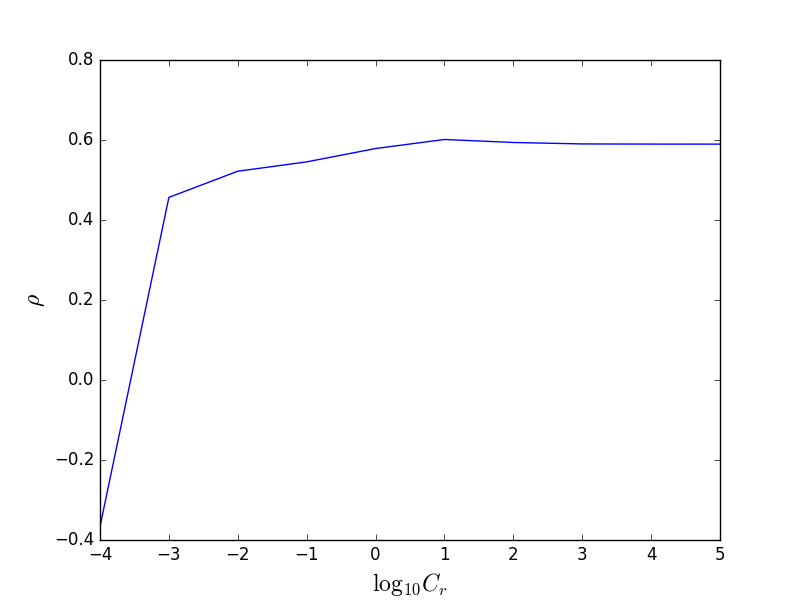
\includegraphics[width=5cm]{plots/pearsonr}}
    \subfloat[]{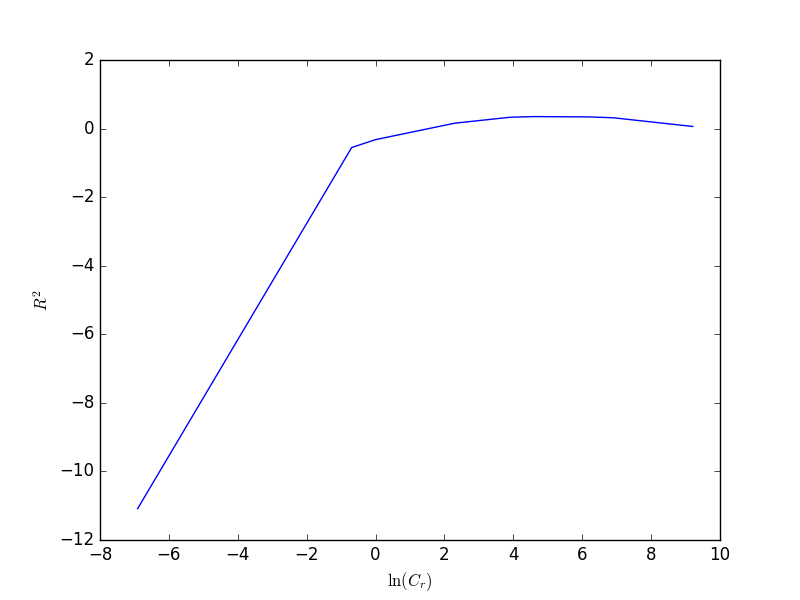
\includegraphics[width=5cm]{plots/r2}}
    \subfloat[]{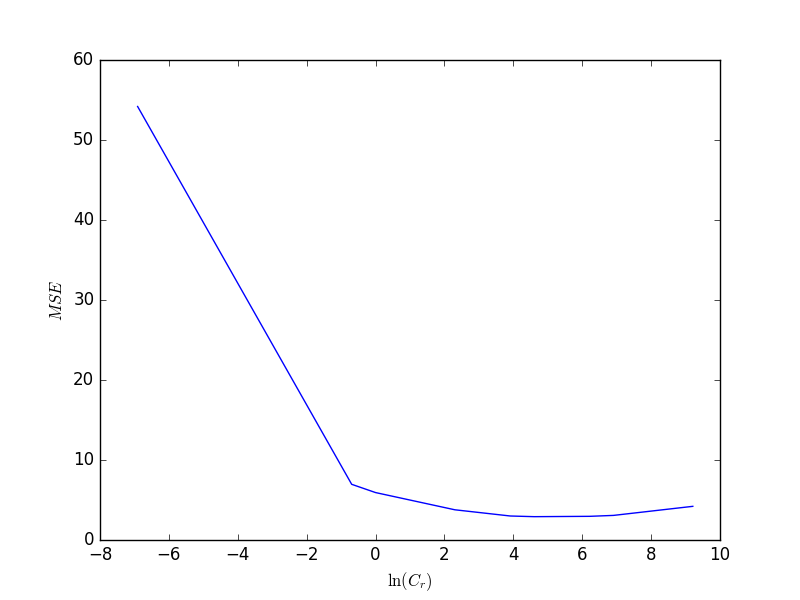
\includegraphics[width=5cm]{plots/mse}}
    \caption{Зависимость (a) коэффициента корреляции Пирсона $\rho$, (b) коэффициента детерминации $R^2$, (c) среднеквадратичной ошибки $MSE$ от значения логарифма коэффициента регуляризации $C_r$.}
    \label{fig1}
\end{figure}

Для значения $C_r = 100$ и $C = 20000$ были проведены тесты на классификацию поз новых соединений. Для этого использовался докинг-тест из бенчмарка CASF, в котором предсказывается правильность угадывания top 1,2,3 поз с RMSD $< 1,2,3$ по сравнению с нативной позой для 195 комплексов белков и лигандов, для каждого из которых авторами теста сгенерировано около 100 поз с RMSD $\leq 10.0$. В отличие от декоев из PDBBind, которые сгенерированы поворотами и трансляцией, в этом тесте декои сгенерированы более сложными докинг-алгоритмами. В скоринг-тесте считается коэффициент корреляции Пирсона между предсказанными скорами 195 комплексов (в нативных конформациях) и известными $log K_i$ или $K_d$. Полученные результаты приведены в Таблице 1 (t1 native $-$ процент комплексов, для которых угаданная поза является нативной. t3q3 $-$ процент комплексов, для которых первые три позы с наилучшим скором оказались в пределах RMSD=3 Ангстрема по сравнению с нативной позой).

\begin{table}[h]
 \begin{tabular}{||c || c || c || c || c || c || c||} 
 \hline
 t1 native 28.2	& t1q1 64.1	& t1q2 72.3	& t1q3 77.4 & t1q1n 55.9 & t1q2n 67.2	& t1q3n 73.3 \\
 \hline
 t2 native 46.7	& t2q1 78.5	& t2q2 84.1	& t2q3 88.2 & t2q1n 68.7 & t2q2n 78.5 & t2q3n 85.1 \\
 \hline
 t3 native 56.9 & t3q1 83.1 & t3q2 88.7	& t3q3 92.3 & t3q1n 73.3 & t3q2n 84.1 & t3q3n 90.3 \\
 \hline
\end{tabular}
\caption{\label{tab:table-name} Результаты на докинг-тесте из бенчмарка CASF}
\end{table}

В данном тесте коэффициент корреляции Пирсона составил $\rho=0.521182$.

\section{Заключение}
Полученная модель показала достойные результаты на докинг-тестах из бенчмарка CASF, однако результаты могут быть выше, если точнее подобрать коэффициенты регуляризации и работать с данными повышенной размерности. Предлагается расширить признаковое описание комплексов, добавив дополнительные водные дескрипторы, а также признаки, определяющие количества связей в комплексе и их вращения.

% С помощью кросс-валидации было подобрано значение коэффициента регуляризации $C=1024$, а методом перебора было получено оптимальное значение коэффициента регуляризации $C_r = 100$.

% С помощью полученной модели были предсказаны значения постоянной аффинности для нативных поз тестовой выборки. Корреляция между истинными и предсказанными значениями оказалась равна $\rho=0.6201$ с p-значением $p=2.6774\times 10^{-133}$, коэффициент детерминации $R^2=-0.2094$, среднеквадратичное отклонение $\text{MSE}=5.4160$.

%% References
%%
%% Following citation commands can be used in the body text:
%% Usage of \cite is as follows:
%%   \cite{key}         ==>>  [#]
%%   \cite[chap. 2]{key} ==>> [#, chap. 2]
%%

%% References with bibTeX database:

\bibliographystyle{elsarticle-num}
%bibliographystyle{elsarticle-harv}
% \bibliographystyle{elsarticle-num-names}
% \bibliographystyle{model1a-num-names}
% \bibliographystyle{model1b-num-names}
% \bibliographystyle{model1c-num-names}
% \bibliographystyle{model1-num-names}
% \bibliographystyle{model2-names}
% \bibliographystyle{model3a-num-names}
% \bibliographystyle{model3-num-names}
% \bibliographystyle{model4-names}
% \bibliographystyle{model5-names}
% \bibliographystyle{model6-num-names}

\begin{thebibliography}{4}
\bibitem{virtual_screening} 
Christoph Sotriffer and Hans Matter. 
\textbf{Virtual Screening: Principles, Challenges, and Practical Guidelines}. 
Wiley Online Library, 10.1002/9783527633326.ch7 edition, 2011.
 
\bibitem{docking} 
Lengauer T, Rarey M (Jun 1996).  
\textbf{"Computational methods for biomolecular docking". Current Opinion in Structural Biology}. 
6 (3): 402–6.
 
\bibitem{classification} 
Maria Kadukova, Sergei Grudinin.
\textbf{Convex-PL: a novel knowledge-based potential for protein-ligand interactions deduced from structural databases using convex optimization}.
Journal of Computer-Aided Molecular Design, October 2017, Volume 31, Issue 10, pp 943–958.

\bibitem{scoring_functions} 
Xuan-Yu Meng, Hong-Xing Zhang, Mihaly Mezei, and Meng Cui.
\textbf{Molecular Docking: A powerful approach for structure-based drug discovery}.
Curr Comput Aided Drug Des. 2011 Jun 1; 7(2): 146–157.

\bibitem{convex_optimization} 
S.P. Boyd and L. Vandenberghe.
\textbf{Convex optimization}.
Cambridge Univ Press, 2004.

\bibitem{vapnik} 
V. Vapnik.
\textbf{The nature of statistical learning theory}.
Springer, 2000.

\bibitem{D3R}
Maria Kadukova and Sergei Grudinin.
\textbf{Docking of small molecules to farnesoid X receptors using AutoDock Vina with the Convex-PL potential : lessons learned from D3R Grand Challenge 2}.
J. Comput.-Aided Mol. Des., 2017. 

\bibitem{regression} 
Sergei Grudinin, Maria Kadukova, Andreas Eisenbarth, Simon Marillet, Frédéric Cazals.
\textbf{Predicting binding poses and affinities for protein-ligand complexes in the 2015 D3R Grand Challenge using a physical model with a statistical parameter estimation}.
J Comput Aided Mol Des. 2016 Sep;30(9):791-804. Epub 2016 Oct 7.

\bibitem{KRR1} 
D. Barber.
\textbf{Bayesian reasoning and machine learning}.
Cambridge University Press, Cambridge, 2012.

\bibitem{KRR2} 
Kevin Vu, John Snyder, Li Li, Matthias Rupp, Brandon F. Chen, Tarek Khelif, Klaus-Robert Müller, Kieron Burke.
\textbf{Understanding Kernel Ridge Regression: Common behaviors from simple functions to density functionals}.

\bibitem{KRR3} 
Press, WH; Teukolsky, SA; Vetterling, WT; Flannery, BP (2007).
\textbf{"Section 19.5. Linear Regularization Methods". Numerical Recipes: The Art of Scientific Computing (3rd ed.)}.
New York: Cambridge University Press. ISBN 978-0-521-88068-8.

\bibitem{rmax1} 
Sheng-You Huang and Xiaoqin Zou.
\textbf{An iterative knowledge-based scoring function for protein–protein recognition}.
Proteins: Struct., Funct., Bioinf., 72(2):557–579, 2008.

\bibitem{rmax2} 
Gwo-Yu Chuang, Dima Kozakov, Ryan Brenke, Stephen R Comeau, and Sandor Vajda.
\textbf{Dars (decoys as the reference state) potentials for protein-protein docking}.
Biophys. J., 95(9):4217–4227, 2008.

\bibitem{rmax3} 
Vladimir N Maiorov and Gordon M Grippen.
\textbf{Contact potential that recognizes the correct folding of globular proteins}.
J. Mol. Biol., 227(3):876–888, 1992.

\bibitem{rmax4} 
Jian Qiu and Ron Elber.
\textbf{Atomically detailed potentials to recognize native and approximate protein structures}.
Proteins: Struct., Funct., Bioinf., 61(1):44–55, 2005.

\bibitem{rmax5} 
Dror Tobi and Ivet Bahar.
\textbf{Optimal design of protein docking potentials: Efficiency and limitations}.
Proteins: Struct., Funct., Bioinf., 62(4):970–981, 2006.

\bibitem{rmax6} 
Myong-Ho Chae, Florian Krull, Stephan Lorenzen, and Ernst-Walter Knapp.
\textbf{Predicting protein complex geometries with a neural network}.
Proteins: Struct., Funct., Bioinf., 78(4):1026–1039, 2010.

\bibitem{PDB1} 
Renxiao Wang, Xueliang Fang, Yipin Lu, Chao-Yie Yang, and Shaomeng Wang.
\textbf{The PDBbind Database: Methodologies And Updates}.
J. Med. Chem., 48(12):4111–9, June 2005.

\bibitem{PDB2} 
Renxiao Wang, Xueliang Fang, Yipin Lu, and Shaomeng Wang.
\textbf{The PDBbind Database: Collection of Binding Affinities for Protein-Ligand Complexes with Known Three-Dimensional Structures}.
J. Med. Chem., 47(12):2977–80, June 2004.

\bibitem{liblinear} 
Rong-En Fan, Kai-Wei Chang, Cho-Jui Hsieh, Xiang-Rui Wang, Chih-Jen Lin.
\textbf{LIBLINEAR: A Library for Large Linear Classification}.
The Journal of Machine Learning Research archive, Volume 9, 6/1/2008, Pages 1871-1874.

\bibitem{dualSVM} 
Cho-Jui Hsieh, Kai-Wei Chang, Chih-Jen Lin, S. Sathiya Keerthi, and Sellamanickam Sundararajan.
\textbf{ A dual coordinate descent method for large-scale linear SVM}.
In Proceedings
of the Twenty Fifth International Conference on Machine Learning (ICML), 2008.

\end{thebibliography}

\end{document}

%%
%% End of file `elsarticle-template-num.tex'.
